%CHAPTER 1
\chapter{HỆ THỐNG THÔNG TIN TRONG NGỮ CẢNH LOGIC MÔ TẢ}
\label{chap:chapter1}
Logic mô tả (Description Logics - DLs) là một họ các ngôn ngữ hình thức được sử dụng để biểu diễn và suy luận tri thức trong một miền ứng dụng cụ thể. Logic mô tả biểu diễn các thuật ngữ thông qua các đối tượng, khái niệm và vai trò.
%
Bắt đầu từ các khái niệm nguyên tử, vai trò nguyên tử, logic mô tả cho phép xây dựng các khái niệm phức, vai trò phức bằng cách sử dụng các khái niệm nguyên tử, vai trò nguyên tử cùng với tập các tạo tử đã cho. Một hệ thống logic mô tả cho phép mô tả các khái niệm có liên quan với nhau và các tri thức tiềm ẩn. Các tri thức tiềm ẩn này có thể được suy luận từ những tri thức đã được biểu diễn thông qua các dịch vụ suy luận hoặc các bộ suy luận.

\section{Giới thiệu về logic mô tả}
\label{chap1.sec:Introduction}
Thuật ngữ {\em logic mô tả}, được sử dụng rộng rãi từ năm 1984. Ban đầu logic mô tả được sử dụng để biểu diễn tri thức bởi Quillian vào năm 1967 thông qua thuật ngữ {\em mạng ngữ nghĩa} (semantic networks) và Minsky vào năm 1981 với thuật ngữ {\em hệ thống khung} (frame systems). Năm 1985, hệ thống \textsc{KL-one}~\cite{ref:Brachman} ra đời đã đưa ra một định hướng nghiên cứu cho logic mô tả. 

Logic mô tả dựa vào tập ký hiệu các tên cá thể (có thể hiểu như là các đối tượng, các hằng), tên khái niệm (có thể hiểu như là các lớp, các vị từ một đối), các tên vai trò (có thể hiểu như là các quan hệ hai ngôi, các vị từ hai đối) và tập các tạo tử đặc trưng cho phép tạo nên các khái niệm phức, vai trò phức từ các khái niệm nguyên tử ({\em bao gồm khái niệm nguyên thủy và khái niệm định nghĩa}) và vai trò nguyên tử ({\em bao gồm vai trò nguyên thủy và vai trò định nghĩa}).

\begin{Example}\label{chap1.ex:PrimitiveConcept}
Giả sử chúng ta có các khái niệm nguyên thủy và vai trò nguyên thủy sau:

  \begin{tabular}{l l}
   $\mathsf{Human}$ & là khái niệm để chỉ các đối tượng là người\\
   $\mathsf{Female}$ & là khái niệm để chỉ các đối tượng là giống cái\\
%   $\mathsf{Male}$ & là khái niệm để chỉ các đối tượng là giống đực\\
   $\mathsf{Rich}$ & là khái niệm để chỉ những đối tượng giàu có\\
   $\mathsf{hasChild}$ & là vai trò để chỉ đối tượng này có con là đối tượng kia\\
   $\mathsf{marriedTo}$ & là vai trò để chỉ đối tượng này kết hôn với đối tượng kia \hspace{10.5ex} \myend
  \end{tabular}
\end{Example}

\begin{Example}\label{chap1.ex:ComplexConcept}
Với những khái niệm nguyên thủy, vai trò nguyên thủy đã cho trong Ví dụ~\ref{chap1.ex:PrimitiveConcept} và các tạo tử {\em phủ định của khái niệm} ($\neg$), {\em giao của các khái niệm} ($\mand$), {\em hợp của các khái niệm} ($\mor$), {\em lượng từ hạn chế tồn tại} ($\E$), {\em lượng từ hạn chế với mọi} ($\V$), chúng ta có thể xây dựng các khái niệm phức sau:

  \begin{tabular}{l}
%    \hline   
    $\mathsf{Human \mand Female}$\\
    \qquad là khái niệm để chỉ các đối tượng là người phụ nữ\\
    $\mathsf{Human \mand \neg Female}$\\
    \qquad là khái niệm để chỉ các đối tượng là người đàn ông\\
    $\mathsf{Human \mand \E hasChild.(Human \mand Female)}$\\
    \qquad là khái niệm để chỉ các đối tượng là cha mẹ có con gái\\
    $\mathsf{Human \mand \E marriedTo.Human}$\\
    \qquad là khái niệm để chỉ những người đã kết hôn\\ 
    $\mathsf{Human \mand \V hasChild.Female}$\\
    \qquad là khái niệm để chỉ những người chỉ có toàn con gái\\
    $\mathsf{Female \mand Rich}$\\
    \qquad là khái niệm để chỉ những phụ nữ giàu có \hspace{33.0ex}\myend
%    \hline
  \end{tabular}
\end{Example}

Thông tin trong các hệ thống logic mô tả được lưu trữ thông qua một {\em cơ sở tri thức}. Thông thường, một cơ sở tri thức gồm có hai thành phần: {\em TBox}, còn gọi là {\em bộ thuật ngữ}, và {\em ABox}, còn được gọi là {\em bộ khẳng định}. Từ cơ sở tri thức, người ta có thể xây dựng một hệ thống logic mô tả để thực hiện việc biểu diễn và suy luận thông tin. Thông thường, một cơ sở tri thức gồm có các thành phần sau:~\cite{ref:Baader00}

\begin{figure}[h]\label{chap1.fig:KnowledgeBase}
  \setlength{\unitlength}{1cm}
  \begin{picture}(15, 5.5)(0,0)
    \put(1.9,2.8){\circle{3}}
    \put(1.6,2.65){\text{\textbf{DL}}}
    \put(0.8,1.8){\text{\textbf{Logic mô tả}}}
    \put(2.0,2.1){\vector(1,-2){1.0}}
    \put(2.0,3.5){\vector(1,2){1.0}}
    
    \put(3,0){\framebox(7,5.5)}
    \put(3.9,4.5){\text{\textbf{CƠ SỞ TRI THỨC - KB}}}
    
    \put(3.5,0.5){\framebox(6,1.5)}
    \put(4.1,1.0){\text{\textbf{ABox - Bộ khẳng định}}}
    
    \put(3.5,2.5){\framebox(6,1.5)}
    \put(4.2,3.0){\text{\textbf{TBox - Bộ thuật ngữ}}}
    
    \put(10.0,4.0){\vector(1,0){1.0}}
    \put(11.0,3.0){\vector(-1,0){1.0}}
    \put(10.0,2.0){\vector(1,0){1.0}}
    \put(11.0,1.0){\vector(-1,0){1.0}}
    
    \put(11,0){\framebox(1,5.5)}
    \put(11.35,5.05){\text{H}}
    \put(11.35,4.65){\text{Ệ}}
    
    \put(11.35,4.20){\text{T}}
    \put(11.35,3.85){\text{H}}
    \put(11.35,3.45){\text{Ố}}
    \put(11.35,3.10){\text{N}}
    \put(11.35,2.75){\text{G}}
    
    \put(11.40,2.40){\text{S}}
    \put(11.35,2.05){\text{U}}
    \put(11.35,1.70){\text{Y}}
    
    \put(11.38,1.30){\text{L}}
    \put(11.35,0.95){\text{U}}
    \put(11.35,0.55){\text{Ậ}}
    \put(11.35,0.15){\text{N}}
    
    \put(12.0,4.5){\vector(1,0){1.0}}
    \put(13.0,3.5){\vector(-1,0){1.0}}
    \put(12.0,2.5){\vector(1,0){1.0}}
    \put(13.0,1.5){\vector(-1,0){1.0}}
    
    \put(13,0){\framebox(1,5.5)}
    \put(13.35,4.05){\text{\textbf{G}}}
    \put(13.42,3.65){\text{\textbf{I}}}
    \put(13.35,3.20){\text{\textbf{A}}}
    \put(13.35,2.85){\text{\textbf{O}}}

    \put(13.35,2.10){\text{\textbf{D}}}
    \put(13.42,1.75){\text{\textbf{I}}}
    \put(13.35,1.35){\text{\textbf{Ệ}}}
    \put(13.35,0.95){\text{\textbf{N}}}
    
    \put(15.0,3.0){\vector(-1,0){1.0}}
    \put(14.0,2.0){\vector(1,0){1.0}}
    
  \end{picture}
\caption{Kiến trúc của một hệ cơ sở tri thức trong logic mô tả}
\end{figure}

\begin{itemize}
  \item \textbf{Bộ thuật ngữ ({\em Terminology Box - TBox})}: Bộ thuật ngữ chứa các tiên đề về thuật ngữ, nó cho phép xây dựng các khái niệm phức từ những khái niệm nguyên tử và vai trò nguyên tử,\ldots Bên cạnh đó, bộ thuật ngữ còn cho biết mối quan hệ giữa các khái niệm thông qua các tiên đề bao hàm khái niệm tổng quát, tiên đề tương đương khái niệm,\ldots Chúng ta xét ví dụ sau về mối quan hệ giữa các con người với nhau thông qua bộ thuật ngữ.
\end{itemize}
  
\begin{Example}\label{chap1.ex:TBox}
  Với các khái niệm nguyên thủy đã cho ở trong Ví dụ~\ref{chap1.ex:PrimitiveConcept}, chúng ta có thể xây dựng bộ thuật ngữ như sau:
  
  \begin{tabular}{l}
%  \hline
  $\mathsf{Parent = Human \mand \E hasChild.Human \mand \V hasChild.Human}$\\
  $\mathsf{Male = Human \mand \neg Female}$\\
  $\mathsf{Husband = Male \mand \E marriedTo.Human}$\\
  $\mathsf{Husband \sqsubseteq \V marriedTo.Female}$\\
  $\mathsf{Male \mand Female = \bot}$
%  \hline
  \end{tabular}\label{dádá}

  Ba phát biểu đầu tiên của bộ thuật ngữ dùng để định nghĩa các khái niệm mới đó là $\mathsf{Parent, Male}$ và $\mathsf{Husband}$ tương ứng dùng để chỉ những đối tượng là bố mẹ, người đàn ông và người chồng. Phát biểu thứ tư yêu cầu mọi thể hiện của $\mathsf{Husband}$ phải thỏa mãn khái niệm $\mathsf{\V marriedTo.Female}$, nghĩa là, mọi người đàn ông đã kết hôn (được gọi là chồng) thì phải kết hôn với một người phụ nữ. Phát biểu cuối cùng để biểu diễn hai khái niệm $\mathsf{Male}$ và $\mathsf{Female}$ không giao nhau. Nói cách khác, hai khái niệm $\mathsf{Male}$ và $\mathsf{Female}$ là rời nhau.\myend
\end{Example}

\begin{itemize}
  \item \textbf{Bộ khẳng định ({\em Assertion Box - ABox})}: Bộ khẳng định chứa những khẳng định về các cá thể bao gồm khẳng định khái niệm, khẳng định vai trò, khẳng định đẳng thức, khẳng định bất đẳng thức, \ldots
\end{itemize}

\begin{Example}\label{chap1.ex:ABox}
  Với các khái niệm nguyên thủy đã cho trong Ví dụ~\ref{chap1.ex:PrimitiveConcept} và các khái niệm được định nghĩa thêm trong Ví dụ~\ref{chap1.ex:TBox}, chúng ta có thể có những khẳng định sau đây:

  \begin{tabular}{l}
%    \hline
    $\mathsf{Human(LAN)}$\\
    $\mathsf{Male(HUNG)}$\\
    $\mathsf{Husband(HAI)}$\\
    $\mathsf{hasChild(LAN, HUNG)}$\\
    $\mathsf{(\neg Female \mand Rich)(HUNG)}$
%    \hline
  \end{tabular}

Khẳng định thứ nhất cho biết cá thể $\mathsf{LAN}$ là một con người, khẳng định thứ hai cho biết cá thể $\mathsf{HUNG}$ là một người đàn ông, khẳng định thứ ba cho biết cá thể $\mathsf{HAI}$ là một người chồng và khẳng định thứ tư cho biết cá thể $\mathsf{LAN}$ có con là cá thể $\mathsf{HUNG}$ và khẳng định cuối cùng cho biết các thể $\mathsf{HUNG}$ là một người đàn ông giàu có.\myend
\end{Example}

\begin{itemize}
  \item \textbf{Hệ thống suy luận ({\em Inference System - IS})}: Hệ thống suy luận cho phép trích rút ra những tri thức tiềm ẩn từ những tri thức đã có được thể trong ABox và TBox. Một trong những bài toán suy luận phổ biến của logic mô tả là kiểm tra tính bao hàm của các khái niệm. Thông qua Ví dụ~\ref{chap1.ex:TBox}, chúng ta có thể thấy rằng cả $\mathsf{Male}$ và $\mathsf{Female}$ đều được bao hàm trong $\mathsf{Human}$. Một bài toán suy luận khác cũng phổ biến trong logic mô tả là kiểm tra thể hiện của một khái niệm. Nghĩa là xác định xem một cá thể có phải là một thể hiện của một khái niệm hay không. Thông qua Ví dụ~\ref{chap1.ex:TBox} và~\ref{chap1.ex:ABox}, chúng ta có thể khẳng định rằng cá thể $\mathsf{LAN}$ là một thể hiện của khái niệm $\mathsf{Parent}$. Chúng ta cũng có thể khẳng định cá thể $\mathsf{HAI}$ không là thể hiện của khái niệm $\mathsf{Female}$. Lý do đưa ra khẳng định này là: $\mathsf{HAI}$ là thể hiện của $\mathsf{Husband}$, mà $\mathsf{Husband}$ là khái niệm được định nghĩa thông qua phát biểu $\mathsf{Husband = Male \mand \E marriedTo.Human}$. Trong lúc đó, $\mathsf{Male \mand Female = \bot}$ chứa trong TBox.

Một điểm lưu ý là, chúng ta không xem một cơ sở tri thức theo {\em giả thiết thế giới đóng} ({\em closed world assumption - CWA}) mà xem nó như là một {\em giả thiết thế giới mở} ({\em open world assumption - OWA}). Nghĩa là, một khẳng định xuất hiện trong ABox thì được cho đó là đúng. Ngược lại, những khẳng định không xuất hiện trong ABox hoặc không thể suy luận được thông qua bộ suy luận thì không được xem đó là sai mà phải được xem như là chưa biết, ngoại trừ việc suy luận ra được khẳng định đó là sai.

  \item \textbf{Giao diện người dùng ({\em User Interface - UI})}: Giao diện người dùng được sử dụng để giao tiếp với người sử dụng, người sử dụng thông qua giao diện người dùng có thể trích rút ra những thông tin từ cơ sở tri thức. Giao diện người dùng được thiết kế tùy thuộc vào từng ứng dụng cụ thể.
\end{itemize}

\section{Logic mô tả \ALC}
Logic mô tả \ALC\ được Schmidt-Schau\ss và Smolka giới thiệu năm 1991 qua bài báo {\em Attributive Concept Descriptions with Complements} và được xem như là một logic mô tả cơ bản nhất. Logic mô tả \ALC\ cho phép xây dựng các khái niệm phức từ các khái niệm nguyên tử và vai trò nguyên tử bằng cách sử dụng các tạo tử $\mand$ (phép giao), $\mor$ (phép hợp) và $\neg$ (phép phủ định). Hơn nữa, các khái niệm còn được xây dựng thông qua các lượng từ hạn chế phổ quát và lượng từ hạn chế tồn tại đối với các vai trò.

Các Logic mô tả khác được phát triển sau này đều dựa vào logic mô tả \ALC\ và thêm vào các tạo tử khác để xây dưng các logic mô tả phức tạp hơn, có khả năng khả năng biểu diễn tốt hơn. Do vậy, trong phần này, chúng tôi trình bày về logic mô tả \ALC\ cũng như các khái niệm về bài toán suy luận với \ALC.

\begin{Definition}[\textbf{Cú pháp của \ALC}]
\label{chap1.def:SyntaxALC}
Cho $N_C$ là tập các tên khái niệm (khái niệm nguyên tử) và $N_R$ là tập các tên vai trò (vai trò nguyên tử) đôi một không giao nhau. Các khái niệm trong \ALC\ được định nghĩa một cách đệ quy như sau:
\begin{itemize}
  \item $\top$ là một khái niệm của \ALC\ (gọi là khái niệm đỉnh)
  \item $\bot$ là một khái niệm của \ALC\ (gọi là khái niệm đáy)
  \item Nếu $A \in N_C$ thì $A$ là một khái niệm của \ALC
  \item Nếu $C, D$ là các khái niệm của \ALC\ và $r \in N_R$ thì
  \begin{itemize}
    \item $C \mand D$ (giao của hai khái niệm)
    \item $C \mor D$ (hợp của hai khái niệm)
    \item $\neg C$ (Phủ định của khái niệm)
    \item $\E r.C$ (hạn chế tồn tại đầy đủ)
    \item $\V r.C$ (hạn chế phổ quát)
  \end{itemize}
  là các khái niệm của \ALC.\myend
\end{itemize}
\end{Definition}
%-----------------------------------------------------------------
Sau đây là các quy tắc mô tả một cách ngắn gọn hơn về cú pháp của \ALC:
\begin{equation*}
C, D \rightarrow A \mid \top \mid \bot \mid \neg C \mid C \mand D \mid C \mor D \mid \E r.C \mid \V r.C
\end{equation*}

\begin{Definition}[\textbf{Ngữ nghĩa của \ALC}]
\label{def:SemanticALC}

Một diễn dịch $\mI = \tuple{\Delta^\mI, \cdot^\mI}$ gồm một tập không rỗng $\Delta^\mI$, gọi là \textnormal{miền} của $\mI$, và một hàm $\cdot^\mI$, gọi là \textnormal{hàm diễn dịch} của $\mI$, ánh xạ mỗi tên khái niệm $A$ thành một tập con $A^\mI \subseteq \Delta^\mI$, mỗi tên vai trò $r$ thành một quan hệ hai ngôi $r^\mI \subseteq \Delta^\mI \times \Delta^\mI$.
\end{Definition}

\begin{figure}[h]
  \begin{center}
    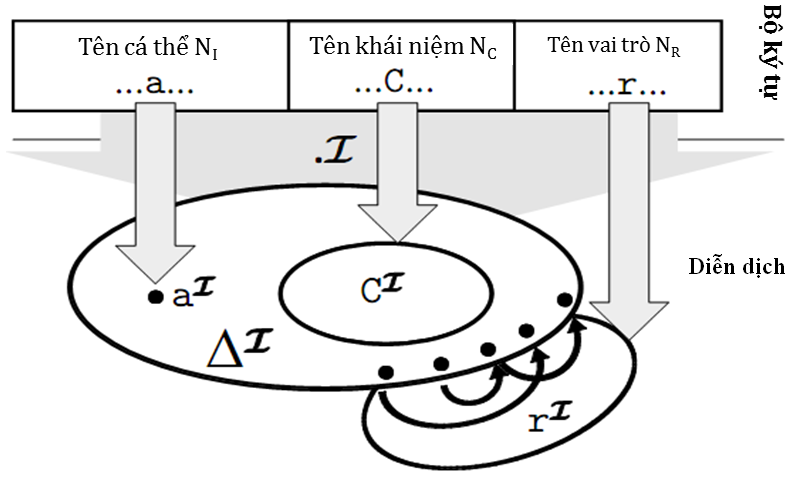
\includegraphics[scale=0.4]{Images/NguNghia.png}
    \caption{Ngữ nghĩa của logic mô tả}\label{fig:Semantic}
  \end{center}
  
\end{figure}

Ngoài ra, ngữ nghĩa của các khái niệm phức có thể được xác định như Hình~\ref{fig:SemanticALC}.

\begin{figure}
  \begin{center}
    \begin{tabular}{|l c l|}
      \hline
      $\top^\mI$ &\!\!\!\!=\!\!\!\!& $\Delta^\mI$\\
      $\bot^\mI$ &\!\!\!\!=\!\!\!\!& $\emptyset$\\
      $\neg C^\mI$ &\!\!\!\!=\!\!\!\!& $\Delta^\mI \setminus C^\mI$\\
      $(C \mand D)^\mI$ &\!\!\!\!=\!\!\!\!& $C^\mI \cap D^\mI$\\
      $(C \mor D)^\mI$ &\!\!\!\!=\!\!\!\!& $C^\mI \cup D^\mI$\\
      $(\V r.C)^\mI$ &\!\!\!\!=\!\!\!\!& $\{x \in \Delta^\mI \mid \V y \mid \tuple{x, y} \in r^\mI \rightarrow y\in C^\mI\}$\\
      $(\E r.C)^\mI$ &\!\!\!\!=\!\!\!\!& $\{x \in \Delta^\mI \mid \E y \mid \tuple{x, y} \in r^\mI \wedge y\in C^\mI\}$\\
    
    \hline
    \end{tabular}
    \caption{Ngữ nghĩa các khái niệm phức của logic mô tả \ALC}\label{fig:SemanticALC}
  \end{center}
  
\end{figure}


\section{Suy luận trong logic mô tả}

\section{Hệ thống thông tin trong ngữ cảnh logic mô tả}

\section{Biểu diễn thông tin trong logic mô tả}

